\documentclass[
]{jss}

%% recommended packages
\usepackage{orcidlink,thumbpdf,lmodern}

\usepackage[utf8]{inputenc}

\author{
Hanne I. Oberman\\Methodology and Statistics\\
Utrecht University \And Johanna Muñoz\\Julius Center for Health Sciences
and Primary Care,\\
University Medical Center Utrecht, Utrecht University,\\
Utrecht, The Netherlands \AND Thomas P. A. Debray\\Julius Center
for Health Sciences and Primary Care,\\
University Medical Center Utrecht, Utrecht University,\\
Utrecht, The Netherlands \And Gerko Vink\\Methodology and Statistics\\
Utrecht University \AND Valentijn M. T. de Jong\\Julius Center for
Health Sciences and Primary Care,\\
University Medical Center Utrecht, Utrecht University,\\
Utrecht, The Netherlands\\
Data Analytics and Methods Task Force,\\
European Medicines Agency,\\
Amsterdam, The Netherlands
}
\title{Imputation of Incomplete Multilevel Data with \proglang{R}}

\Plainauthor{Hanne I. Oberman, Johanna Muñoz, Thomas P. A. Debray, Gerko
Vink, Valentijn M. T. de Jong}
\Plaintitle{Imputation of Incomplete Multilevel Data with R}
\Shorttitle{Multilevel \pkg{mice}}


\Abstract{
This tutorial illustrates the imputation of incomplete multilevel data
with the \proglang{R} packackage \pkg{mice}. Our scope is only simple
multilevel models, to show how imputation can yield less biased
estimates from incomplete clustered data. More complex models can be
accomodated, but are outside the scope of this paper. Incomplete
multilevel data requires careful consideration of the missing data
problem and analysis strategy. In this tutorial, we focus on a popular
strategy for accommodating missingness in multilevel data: replacing the
missing data with one or more plausible values, i.e.,
imputation.Imputation separates the missing data problem from the main
analysis and the completed data can be analyzed as if it has been fully
observed.This tutorial illustrates the imputation of incomplete
multilevel data with the statistical programming language R. We aim to
show how imputation can yield less biased estimates from incomplete
clustered data. We provide practical guidelines and code snippets for
different missing data situations, including non-ignorable missingness
mechanisms. For brevity, we focus on multilevel imputation using chained
equations with the R mice package and its adjacent packages.
}

\Keywords{missing
data, multilevel, clustering, \pkg{mice}, \proglang{R}}
\Plainkeywords{missing data, multilevel, clustering, mice, R}

%% publication information
%% \Volume{50}
%% \Issue{9}
%% \Month{June}
%% \Year{2012}
%% \Submitdate{}
%% \Acceptdate{2012-06-04}

\Address{
    Hanne I. Oberman\\
    Methodology and Statistics\\
Utrecht University\\
    Padualaan 14\\
3584 CH Utrecht\\
  E-mail: \email{h.i.oberman@uu.nl}\\
  URL: \url{https://hanneoberman.github.io/}\\~\\
          }


% tightlist command for lists without linebreak
\providecommand{\tightlist}{%
  \setlength{\itemsep}{0pt}\setlength{\parskip}{0pt}}

% From pandoc table feature
\usepackage{longtable,booktabs,array}
\usepackage{calc} % for calculating minipage widths
% Correct order of tables after \paragraph or \subparagraph
\usepackage{etoolbox}
\makeatletter
\patchcmd\longtable{\par}{\if@noskipsec\mbox{}\fi\par}{}{}
\makeatother
% Allow footnotes in longtable head/foot
\IfFileExists{footnotehyper.sty}{\usepackage{footnotehyper}}{\usepackage{footnote}}
\makesavenoteenv{longtable}


\usepackage{graphicx}
\usepackage{mathtools}
\usepackage{ulem}

\usepackage{amsmath}

\begin{document}



\hypertarget{introduction}{%
\section{Introduction}\label{introduction}}

\hypertarget{multilevel-data}{%
\subsection{Multilevel data}\label{multilevel-data}}

Many datasets include individuals that are clustered together, for
example in geographic regions, or even different studies. In the
simplest case, individuals (e.g., students) are nested within a single
cluster (e.g., school classes). More complex clustered structures may
occur when there are multiple hierarchical levels (e.g., students in
different schools or patients within hospitals within regions across
countries), or when the clustering is non-nested (e.g., electronic
health record data from diverse settings and populations within large
databases). With clustered data we generally assume that individuals
from the same cluster tend to be more similar than individuals from
other clusters. In statistical terms, this implies that observations
from the same cluster are not independent and may in fact be correlated.
If this correlation is left unaddressed, estimates of \emph{p} values,
confidence intervals even model parameters are prone to bias
\citep{loca01}. Statistical methods for clustered data typically adopt
hierarchical models that explicitly describe the grouping of
observations. These models are also known as `multilevel models',
`hierarchical models', `mixed effect models', `random effect models',
and in the context of time-to-event data as `frailty models'. Table
\ref{tab:clus} provides an overview of some key concepts in multilevel
modeling.

Table 1: Concepts in multilevel methods

\begin{CodeChunk}
\begin{table}

\caption{\label{tab:clus0}Concepts in multilevel methods}
\centering
\begin{tabular}[t]{>{\raggedright\arraybackslash}p{3cm}>{\raggedright\arraybackslash}p{12cm}}
\toprule
Concept & Details\\
\midrule
Sample units & Units of the population from which measurements are taken in a sample, e.g., students.\\
Cluster & Variable that specify the cluster or agruppation, e.g., Classroom\\
Hierarchical data & Data are grouped into clusters at different levels, observations belonging to the same cluster are expected to share certain characteristics.\\
Level-1 & Variable that varies within a cluster, eg. Test score\\
Level-2 & Variable that does not vary within a cluster but between, e.g. teacher experience.\\
\addlinespace
Hierarchical model & Model accounting for dependant observations relying on certain parameters ( within cluster) which in turn depend on other parameters (between cluster)\\
Fixed effect & Effects that are constant across all sample units, e.g. something that researchers control for and can repeat, such as  a teaching strategy (tutoring after class)\\
Random effect & Effects that are a source of random variation in the data, and whose levels are not fully sampled. e.g. test score tendency during academic year between students due to no controlled factors such as  genetic,family history\\
Mixed effect & Includes fixed and random effects, e.g. the fixed effect would be the treatment effect of a drug and the random effect would be the ID of the hospital where the patient is treated. Multilevel models typically accommodate for variability by including a separate group mean for each cluster e.g random intercept on hospitals. In addition to random intercepts, multilevel models can also include random coefficients and heterogeneous residual error variances across clusters (see e.g. @gelm06, @hox17 and @jong21).\\
ICC & The variability due to clustering is often measured by means of the intraclass coefficient (ICC). The ICC can be seen as the percentage
of variance that can be attributed to the cluster-level, where a high ICC would indicate that a lot of variability is due to the cluster structure.\\
\addlinespace
Stratified intercept & \\
\bottomrule
\end{tabular}
\end{table}

\end{CodeChunk}

\hypertarget{missingness-in-multilevel-data}{%
\subsection{Missingness in multilevel
data}\label{missingness-in-multilevel-data}}

As with any other dataset, clustered datasets may be impacted by
missingness in much the same way. Several strategies can be used to
handle missing data, including complete case analysis and imputation. We
focus on the latter approach and discuss statistical methods for
replacing the missing data with one or more plausible values. Imputation
separates the missing data problem from the analysis and the completed
data can be analyzed as if it were completely observed. It is generally
recommended to impute the missing values more than once to preserve
uncertainty due to missingness and to allow for valid inferences (c.f.
Rubin 1976).

With incomplete clustered datasets we can distinguish between two types
of missing data: sporadic missingness and systematic missingness
\citep{resc13}. Sporadic missingness arises when variables are missing
for some but not all of the units in a cluster \citep{buur18, jola18}.
For example, it is possible that test results are missing for several
students in one or more classes. When all observations are missing
within one or more clusters, data are said to be systematically missing.
Sporadic missingness is visualized in Figure XYZ.

\begin{CodeChunk}
\begin{figure}

{\centering 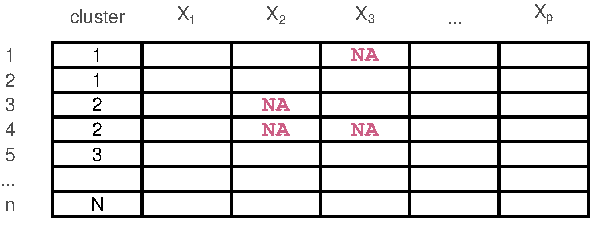
\includegraphics{Imputation_of_Incomplete_Multilevel_Data_files/figure-latex/patterns-1} 

}

\caption[Sporadic missingness in multilevel data]{Sporadic missingness in multilevel data}\label{fig:patterns}
\end{figure}
\end{CodeChunk}

Imputation of missing data requires consideration of the mechanism
behind the missingness. Rubin proposed to distinguish between data that
are missing completely at random (MCAR), data that are missing at random
(MAR) and data that are missing not at random (MNAR; see Table
\ref{tab:miss}). For each of these three missingness generating
mechanisms, different imputation strategies are warranted
(\citet{yuce08} and \citet{hox15}). We here consider the general case
that data are MAR, and expand on certain MNAR situations.

Table 2: Concepts in missing data methods

\begin{longtable}[]{@{}
  >{\raggedright\arraybackslash}p{(\columnwidth - 2\tabcolsep) * \real{0.1739}}
  >{\raggedright\arraybackslash}p{(\columnwidth - 2\tabcolsep) * \real{0.8261}}@{}}
\toprule\noalign{}
\begin{minipage}[b]{\linewidth}\raggedright
\textbf{Concept}
\end{minipage} & \begin{minipage}[b]{\linewidth}\raggedright
\textbf{Details}
\end{minipage} \\
\midrule\noalign{}
\endhead
\bottomrule\noalign{}
\endlastfoot
MCAR & Missing Completely At Random, where the probability to be missing
is equal \\
& across all data entries \\
MAR & Missing At Random, where the probability to be missing depends on
observed \\
& information \\
MNAR & Missing Not At Random (MNAR), where the probability to be
missing \\
& depends on unrecorded information, making the missingness
non-ignorable \\
& \citep{rubi76, meng94}. \\
& \\
\end{longtable}

\hypertarget{aim-of-this-paper}{%
\subsection{Aim of this paper}\label{aim-of-this-paper}}

This papers serves as a tutorial for imputing incomplete multilevel data
with \pkg{mice} in \proglang{R}. \pkg{mice} has become the de-facto
standard for imputation by chained equations, which iteratively solves
the missingness on a variable-by-variable basis. \pkg{mice} is known to
yield valid inferences under many different missing data circumstances
\citep{buur18}.

We provide practical guidelines and code snippets for different missing
data situations, including non-ignorable mechanisms. For reasons of
brevity, we focus on multilevel imputation by chained equations with
\pkg{mice} exclusively; other imputation methods and packages \citep[see
e.g.][ and \citet{grun18}]{audi18} are outside the scope of this
tutorial. Assumed knowledge includes basic familiarity with the
\pkg{lme4} notation for multilevel models (see Table \ref{tab:mod}).

We illustrate imputation of incomplete multilevel data using three case
studies:

\begin{itemize}
\tightlist
\item
  \texttt{popmis} from the \pkg{mice} package \citep[simulated data on
  perceived popularity, \(n = 2,000\) pupils across \(N = 100\) schools
  with data that are MAR,][]{mice};
\item
  \texttt{impact} from the \pkg{metamisc} package \citep[empirical data
  on traumatic brain injuries, \(n = 11,022\) patients across \(N = 15\)
  studies with data that are MAR,][]{metamisc};
\item
  \texttt{obesity} from the \pkg{micemd} package {[}simulated data on
  obesity, \(n = 2,111\) patients across \(N = 5\) regions with data
  that are MNAR{]}.
\end{itemize}

For each of these datasets, we discuss the nature of the missingness,
choose one or more imputation models and evaluate the imputed data, but
we will also highlight one specific aspect of the imputation workflow.

This tutorial is dedicated to readers who are unfamiliar with multiple
imputation. More experienced readers can skip the introduction (case
study 1) and directly head to practical applications of multilevel
imputation under MAR conditions (case study 2) or under MNAR conditions
(case study 3).

\hypertarget{imputation-workflow}{%
\subsection{Imputation workflow}\label{imputation-workflow}}

Below we provide a imputation workflow that can be used in general to
impute cluster data.

\hypertarget{focus-on-the-main-analysis}{%
\subsubsection{Focus on the Main
Analysis}\label{focus-on-the-main-analysis}}

When imputing clustered data, we initially focus on the research
question and the intended analysis, assuming the presence of
non-incomplete values. This assessment sheds light on research
hypotheses and the contemplated main(s) statistical model(s) and it
provides insights into the data's structure (refer to the level table),
variable types (e.g., confounders, auxiliary variables), and other
considerations about variables relationships such as interactions or
polynomial terms.

\hypertarget{exploration-of-available-data}{%
\subsubsection{Exploration of Available
Data}\label{exploration-of-available-data}}

Next, it is necessary to explore the information available in the data.
Exploring individual variables using tools such as histograms or QQ
plots can help to delineate variable distributions and plausible ranges
of values and also identify input errors or outliers. Evaluating
interactions between predictors using scatter plots or conditional
plots, assessing collinearity using VIF or correlations, can help to
glimpse nonlinear relationships that may affect the original formulation
of the main model. Further testing of assumptions related to the
response variable, including variance (homogeneity using conditional box
plots), independence (e.g., ACF, variograms) and response vs.~predictor
relationships (conditional plots - x vs.~y), may serve to choose an
imputation model more suitable to the data. In addition, the intraclass
correlation coefficient (ICC) can be examined to assess cluster
differences, aiding in the choice between the 2l and 1l methods for
imputation.

One can also explore missingness, specifically missing patterns at the
cluster level to identify types of patterns (e.g., non-monotonic,
systematic) to guide the selection of an appropriate imputation approach
in terms of computational efficiency (e.g., simpler regression
imputation versus FCS in univariate patterns). Similarly, these missing
patterns can also be used to identify potential predictors in individual
imputation models by means of inflow criteria (quantifying the
connections between missing data in one variable and other observed
variables) and outflow criteria (determining the connections between
observed values in one variable and missing data in other variables).
Although several packages exist for visualizing missing data, this
tutorial focuses on the recently implemented ggmice package.

\hypertarget{assess-estimation-procedure-robustness-to-missing-data}{%
\subsubsection{Assess Estimation Procedure Robustness to Missing
Data}\label{assess-estimation-procedure-robustness-to-missing-data}}

Prior to implementing multiple imputation, it is critical to assess the
robustness of the estimation model when confronted with missing data.
\cite{Alisson_2002} highlighted scenarios in which specific Maximum
Likelihood (ML) estimation methods outperform Multiple Imputation (MI)
methods. Notably, when the response variable is the sole incomplete
variable, mixed models demonstrate robustness to missing data under the
Missing at Random (MAR) assumption and with a correct
variance-covariance specification.\cite{Molenberghs_2007}. Furthermore,
depending on the proportion of missingness (usually is \textless5\%),
opting for a simpler complete case analysis might be sufficient.

\hypertarget{pre-imputation}{%
\subsubsection{Pre-imputation}\label{pre-imputation}}

Before proceeding with the imputation model, it is necessary to filter
the dataset to include only the minimal variables required for the main
model. If additional procedures are conducted during the analysis, it is
essential to include variables associated with these procedures, such as
confounders in the case of balancing techniques. Other relevant
variables, like instrumental variables or auxiliary variables, may
enhance parameter estimates even if not included in the main model, as
they could be linked to the probability of missingness for some
incomplete variables.

Furthermore, at the variable level, it is crucial to assess whether
proxy variables should be considered or if deterministic imputation
alone is adequate for imputing missing values. For instance, certain
incomplete variables may not necessitate stochastic imputation methods
like MICE. Instead, they can be effectively addressed through deductive
imputation, where incomplete values are inferred from logical and
deterministic relationships between variables. This approach is
especially beneficial for variables that are functions of others, such
as deriving a person's BMI from their weight and height. It also proves
valuable for determining values for one-level variables from two-level
ones, as seen in the context of Individual Participant Data (IPD). In
such cases, incomplete information can be deduced from metadata, like
inferring incomplete data about abortion in a country where abortion is
illegal, or through cross-temporal or protocol-based deduction, such as
imputing missing test values for deceased patients.

\hypertarget{setting-imputation-model}{%
\subsubsection{Setting Imputation
Model}\label{setting-imputation-model}}

\hypertarget{clustering-inclusion}{%
\subparagraph{Clustering Inclusion}\label{clustering-inclusion}}

Various strategies can be employed in the imputation process to account
for clustering, including the inclusion of a cluster indicator variable,
conducting a separate imputation process for each cluster, or employing
a simultaneous imputation method that considers clustering (Stata:
Clustering and MI Impute) TODO: Replace ref.

The choice of strategy depends primarily on the assumptions made in the
main analysis and the constraints imposed by the analyzed
data.Concerning data restrictions, if there are few clusters with many
observations per cluster, the cluster indicator or imputation separated
by groups may be appropriate \cite{Graham_2009}. Conversely, an
imputation model that simultaneously imputes all clusters using a
hierarchical model can be employed when there are more clusters or fewer
observations per cluster \cite{Allison_2002}.

In a hierarchical imputation model, correlations between observations
within clusters are modeled by a random effect, allowing estimation even
with a limited number of observations per cluster. Multiple imputation
models based on hierarchical models have been proposed, each with
different assumptions.

Before choosing a particular strategy, it is crucial to verify if the
assumptions of the imputation model align with those of the main
analysis. For example, using the cluster indicator strategy may
introduce bias estimates when the model is based on a hierarchical
structure \cite{Taaljard_2008}. Even if an imputation strategy congruent
with the main model is preferred, it is essential to assess its
appropriateness for the data, considering that less complex imputation
strategies may lead to unbiased estimates in certain scenarios
\textbackslash cite(Bailey\_2020).

\hypertarget{choice-of-individual-imputation-methods}{%
\paragraph{Choice of Individual Imputation
Methods}\label{choice-of-individual-imputation-methods}}

The initial step involves selecting the individual imputation model for
each incomplete variable in the dataset. The mice package automatically
proposes imputation methods based on the variable type for 1l variables.
For 2l level variables, the micemd package's () function can be
utilized. This function selects among the 2l imputation methods based on
the size of the clusters and the proportion of missingness in each
cluster.

In addition to the package-defined imputation methods, users can specify
custom methods using the ``I formula''. This flexibility allows for the
calculation of derived variables internally or adjustments to imputation
methods based on specific conditions, such as conditioning the
imputation model on the level of an incomplete covariate (e.g.,
pregnancy test on females).

\hypertarget{model-specification}{%
\paragraph{Model Specification}\label{model-specification}}

The imputation model must be congenial with the main model
\cite{Meng_1994}. Congeniality issues arise when the imputation model
and the main model make different assumptions, often due to the omission
of a polynomial or interaction term or the use of transformed variables.

The imputation model can include additional terms than the main model
terms that do not lead to uncongeniality. For instance, it is advisable
to include the outcome variable in the imputation model for prediction
variables \cite{Moons}. In cases where the outcome is time-to-event, the
Nelson-Aalen estimate of the time to the event should be included as a
covariate in the imputation model {[}REF{]}. Furthermore, the inclusion
of auxiliary variables, even if not part of the main model, can be
associated with the probability of missingness, enhancing the likelihood
of satisfying the Missing at Random (MAR) assumption and improving
estimation efficiency \cite{Hardt_2012}.

The specification of imputation models is done on a variable basis,
either using a prediction matrix where the type of prediction variable
should be specified accordingly (see table) or through a list of
formulas in the formula parameter. The latter option proves useful in
formulating imputation models with polynomial terms or interactions
compared to the prediction matrix specification, which requires the
inclusion of additional terms as Just Another Variable (JAV).

However, even when considering an interaction term, depending on the
adapted individual imputation model, it has been suggested, for
instance, for treatment interaction effects, to conduct separated
imputation by treatment group \cite{Zhang_2023}. Additionally, there are
imputation models based on random forest or deep learning that can
handle interaction and non-linear terms that do not require the explicit
inclusion of the non-linear terms.

\hypertarget{post-imputation}{%
\subsubsection{Post-Imputation}\label{post-imputation}}

During the imputation process, certain issues may arise that halt the
process. In hierarchical model imputations, many issues are linked to
methods based on parametric hierarchical models, which may struggle to
estimate a model midway through the process. In such cases, it is
advisable to examine the imputation log file to identify variables with
imputation issues. Subsequently, reducing the number of predictors in
the imputation model could be explored, either by using functions like
quickpred or by considering variable transformations, such as scaling.
Adjusting the level of the hierarchical model (e.g., using a homogenous
variance model or a 1l model) can also be beneficial. Additionally,
checking the range of imputed variables is crucial, as excessively large
imputed values for one predictor could lead to convergence issues in
other variables. This can be mitigated by including post-processing
specifications on problematic variables or by using imputation models
like Predicted Mean Matching (PMM), ensuring imputed values align with
the observable values. In certain cases, a separate imputation strategy
may be considered. For instance, in analyses involving multiple
endpoints, conducting separate imputation processes for each endpoint
might be preferable to a unified imputation process.

\hypertarget{convergence-and-sensitivity-analysis}{%
\subsubsection{Convergence and Sensitivity
Analysis}\label{convergence-and-sensitivity-analysis}}

Before commencing the analysis, it is imperative to verify the
convergence of the imputation process. This is typically achieved
through trace plots or by evaluating prediction plots.

While the majority of Multiple Imputation by Chained Equations (MICE)
methods are based on Missing at Random (MAR) assumptions, field expert
input may suggest that the Missing Not at Random (MNAR) mechanism could
be plausible for certain variables. An MNAR variable is one in which the
probability of missingness depends on an unobservable variable. This can
occur when missingness is associated with the incomplete value itself
(self-marking) or when there is an unobserved variable linked to both
the value and the probability of missingness of the incomplete value
(indirectly non-informative). Specifically, for the indirectly
non-informative case in hierarchical datasets, imputation methods based
on the Heckman method, such as those proposed by Hammon (2021) and Munoz
(2023), can be considered.

\hypertarget{setup}{%
\subsection{Setup}\label{setup}}

Set up the R environment and load the necessary packages:

\begin{CodeChunk}
\begin{CodeInput}
R> set.seed(123)         # for reproducibility
R> library(mice)         # for imputation
R> library(miceadds)     # for additional imputation routines
R> library(ggmice)       # for incomplete/imputed data visualization
R> library(ggplot2)      # for visualization
R> library(dplyr)        # for data wrangling
R> library(lme4)         # for multilevel modeling
R> library(mitml)        # for multilevel parameter pooling
R> library(micemd)       # for case study data and imputation cf. heckman models
R> library(metamisc)     # for case study data
R> library(broom.mixed)  # for multilevel estimates
\end{CodeInput}
\end{CodeChunk}

TODO: add table with predictor matrix values

\begin{itemize}
\tightlist
\item
  -2 = cluster variable
\item
  1 = overall effect
\item
  3 = overall + group-level effect
\item
  4 = individual-level (random) and group-level (fixed) effect
\end{itemize}

\hypertarget{case-study-i-popularity-data}{%
\section{Case study I: popularity
data}\label{case-study-i-popularity-data}}

In this section we will go over the different steps involved with
imputing incomplete multilevel data with the R package mice. We consider
the simulated \texttt{popmis} dataset, which included pupils
(\(n = 2000\)) clustered within schools (\(N = 100\)). The following
variables are of primary interest:

\begin{itemize}
\tightlist
\item
  \texttt{school}, school identification number (clustering variable);
\item
  \texttt{popular}, pupil popularity (self-rating between 0 and 10;
  unit-level);
\item
  \texttt{sex}, pupil sex (0=boy, 1=girl; unit-level);
\item
  \texttt{texp}, teacher experience (in years; cluster-level).
\end{itemize}

The research objective of the \texttt{popmis} dataset is to predict the
pupils' popularity based on their gender and the experience of the
teacher. The analysis model corresponding to this dataset is multilevel
regression with random intercepts, random slopes and a cross-level
interaction. The outcome variable is \texttt{popular}, which is
predicted from the unit-level variable \texttt{sex} and the
cluster-level variable \texttt{texp}:

\begin{CodeChunk}
\begin{CodeInput}
R> mod <- popular ~ 1 + sex + (1 | school)
\end{CodeInput}
\end{CodeChunk}

The estimated effects in the complete data are presented in Table XYZ.
We consider the associations in the full data set to be the true
associations.

Load the data into the environment and select the relevant variables:

\begin{CodeChunk}
\begin{CodeInput}
R> popmis <- popmis[, c("school", "popular", "sex")] 
\end{CodeInput}
\end{CodeChunk}

First we plot the pattern of missing data within categories of the
relevant variables. Plot the missing data pattern:

\begin{CodeChunk}
\begin{CodeInput}
R> plot_pattern(popmis)
\end{CodeInput}
\begin{figure}

{\centering 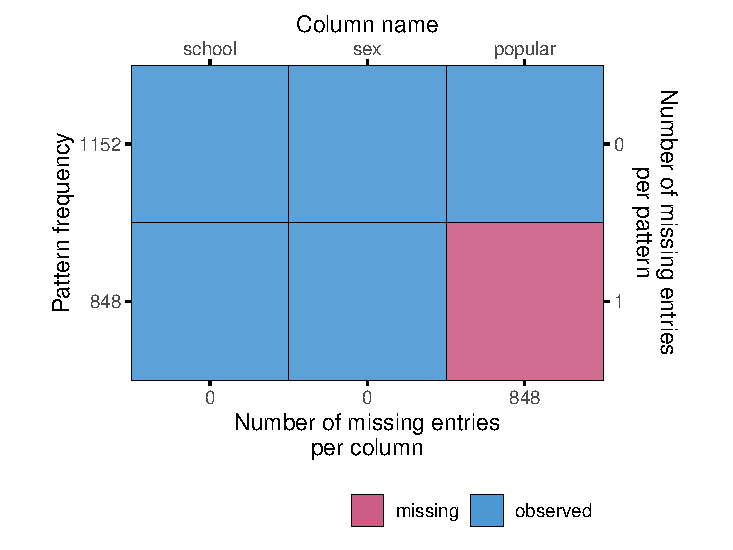
\includegraphics{Imputation_of_Incomplete_Multilevel_Data_files/figure-latex/pop_pat-1} 

}

\caption[Missing data pattern in the popularity data]{Missing data pattern in the popularity data}\label{fig:pop_pat}
\end{figure}
\end{CodeChunk}

The missingness is univariate and sporadic, which is illustrated in the
missing data pattern in Figure \ref{fig:pop_pat}.

The ICC in the incomplete data is
\texttt{round(icc(popular\ \textasciitilde{}\ as.factor(school),\ data\ =\ na.omit(popmis)),\ 2)}.
This tells us that the multilevel structure of the data should probably
be taken into account. If we don't, we'll may end up with incorrect
imputations, biasing the effect of the clusters towards zero.

To develop the best imputation model for the incomplete variable
\texttt{popular}, we need to know whether the observed values of
\texttt{popular} are related to observed values of other variables. Plot
the pair-wise complete correlations in the incomplete data:

\begin{CodeChunk}
\begin{CodeInput}
R> plot_corr(popmis)
\end{CodeInput}


\begin{center}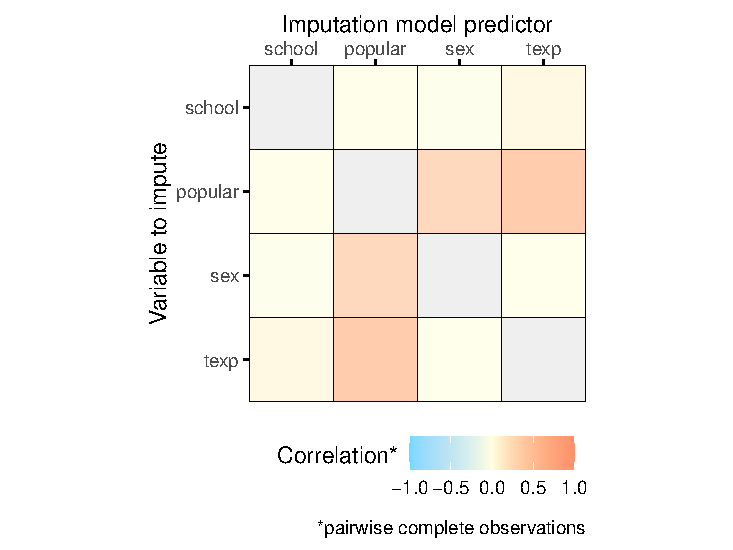
\includegraphics{Imputation_of_Incomplete_Multilevel_Data_files/figure-latex/pop-corr-1} \end{center}

\end{CodeChunk}

This shows us that \texttt{sex} may be a useful imputation model
predictor. Moreover, the missingness in \texttt{popular} may depend on
the observed values of other variables.

\begin{CodeChunk}
\begin{CodeInput}
R> # ggmice(popmis, aes(sex)) +
R> #   geom_histogram(fill = "white") +
R> #   facet_grid(. ~ is.na(popular), scales = "free", labeller = label_both)
R> 
R> ggplot(popmis, aes(y = popular, group = sex)) +
+   geom_boxplot() + 
+   theme_classic()
\end{CodeInput}


\begin{center}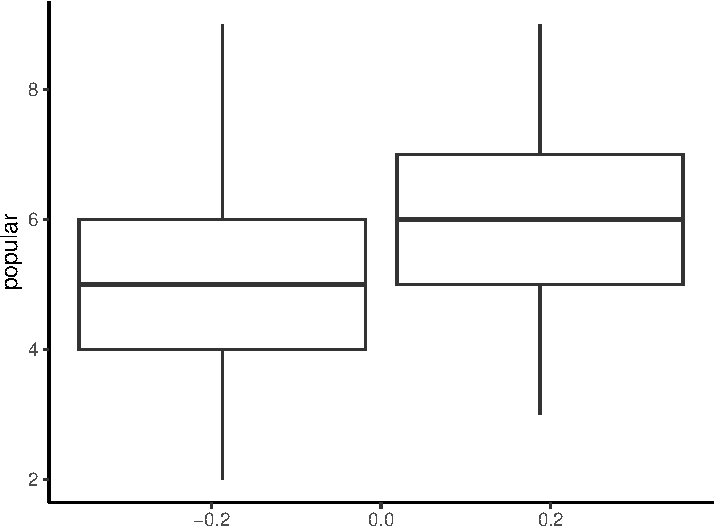
\includegraphics{Imputation_of_Incomplete_Multilevel_Data_files/figure-latex/pop-hist-1} \end{center}

\end{CodeChunk}

\hypertarget{imputation-ignoring-the-cluster-variable-not-recommended}{%
\subsubsection{Imputation ignoring the cluster variable (not
recommended)}\label{imputation-ignoring-the-cluster-variable-not-recommended}}

The first imputation model that we'll use is likely to be invalid. We do
\emph{not} use the cluster identifier \texttt{school} as imputation
model predictor. With this model, we ignore the multilevel structure of
the data, despite the high ICC. This assumes exchangeability between
units. We include it purely to illustrate the effects of ignoring the
clustering in our imputation effort.

Create a methods vector and predictor matrix for \texttt{popular}, and
make sure \texttt{school} is not included as predictor:

\begin{CodeChunk}
\begin{CodeInput}
R> meth <- make.method(popmis) # methods vector
R> pred <- quickpred(popmis)   # predictor matrix
R> plot_pred(pred)
\end{CodeInput}


\begin{center}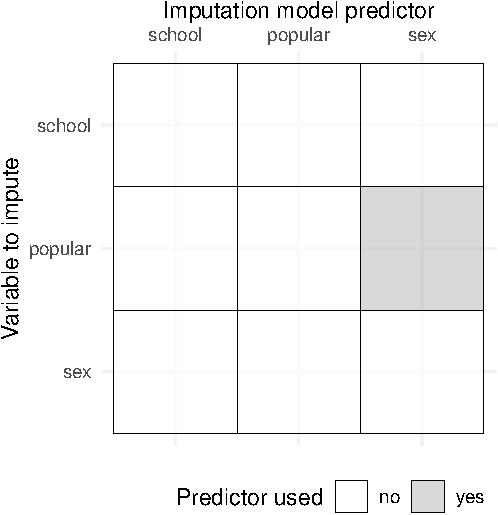
\includegraphics{Imputation_of_Incomplete_Multilevel_Data_files/figure-latex/pop-ignored-pred-1} \end{center}

\end{CodeChunk}

Impute the data, ignoring the cluster structure:

\begin{CodeChunk}
\begin{CodeInput}
R> imp <- mice(popmis, pred = pred, print = FALSE)
\end{CodeInput}
\end{CodeChunk}

Evaluate the convergence of the algorithm:

\begin{CodeChunk}
\begin{CodeInput}
R> plot_trace(imp)
\end{CodeInput}


\begin{center}\includegraphics{Imputation_of_Incomplete_Multilevel_Data_files/figure-latex/pop-ignored-conv-1} \end{center}

\end{CodeChunk}

Analyze the imputations:

\begin{CodeChunk}
\begin{CodeInput}
R> fit <- with(imp, 
+             lmer(popular ~ 1 + sex  + (1 | school))) 
\end{CodeInput}
\end{CodeChunk}

Print the estimates:

\begin{CodeChunk}
\begin{CodeInput}
R> testEstimates(as.mitml.result(fit), extra.pars = TRUE)
\end{CodeInput}
\end{CodeChunk}

\hypertarget{imputation-with-the-cluster-variable-as-predictor-not-recommended}{%
\subsubsection{Imputation with the cluster variable as predictor (not
recommended)}\label{imputation-with-the-cluster-variable-as-predictor-not-recommended}}

We will now use \texttt{school} as a predictor to impute all other
variables. This is still not recommended practice, since it only works
under certain circumstances and results may be biased
\citep{drec15, ende16}. But at least, it includes some multilevel
aspect. This method is also called `fixed cluster imputation', and uses
N-1 indicator variables representing allocation of N clusters as a fixed
factor in the model \citep{reit06, ende16}. Colloquially, this is
`multilevel imputation for dummies'.

\begin{CodeChunk}
\begin{CodeInput}
R> # adjust the predictor matrix
R> pred["popular", "school"] <- 1 
R> plot_pred(pred)
\end{CodeInput}


\begin{center}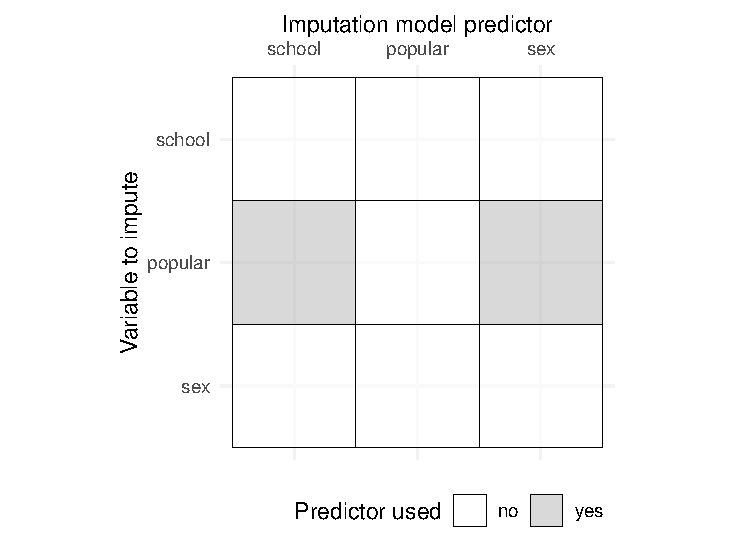
\includegraphics{Imputation_of_Incomplete_Multilevel_Data_files/figure-latex/pop_predictor-1} \end{center}

\begin{CodeInput}
R> # impute the data, cluster as predictor
R> imp <- mice(popmis, pred = pred, print = FALSE)
\end{CodeInput}
\end{CodeChunk}

Evaluate the convergence of the algorithm:

\begin{CodeChunk}
\begin{CodeInput}
R> plot_trace(imp)
\end{CodeInput}


\begin{center}\includegraphics{Imputation_of_Incomplete_Multilevel_Data_files/figure-latex/pop-predictor-conv-1} \end{center}

\end{CodeChunk}

Analyze the imputations:

\begin{CodeChunk}
\begin{CodeInput}
R> fit <- with(imp, 
+             lmer(popular ~ 1 + sex + (1 | school))) 
\end{CodeInput}
\end{CodeChunk}

Print the estimates:

\begin{CodeChunk}
\begin{CodeInput}
R> testEstimates(as.mitml.result(fit), extra.pars = TRUE)
\end{CodeInput}
\end{CodeChunk}

\hypertarget{imputation-with-multilevel-model}{%
\subsubsection{Imputation with multilevel
model}\label{imputation-with-multilevel-model}}

\begin{CodeChunk}
\begin{CodeInput}
R> # adjust the predictor matrix
R> pred["popular", "school"] <- -2 
R> plot_pred(pred)
\end{CodeInput}


\begin{center}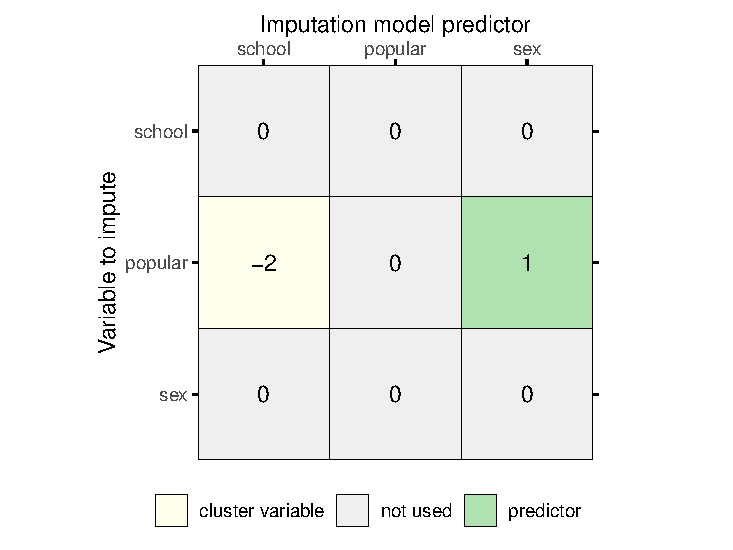
\includegraphics{Imputation_of_Incomplete_Multilevel_Data_files/figure-latex/pop_multilevel-1} \end{center}

\begin{CodeInput}
R> # impute the data, cluster as predictor
R> imp <- mice(popmis, pred = pred, print = FALSE)
\end{CodeInput}
\end{CodeChunk}

Evaluate the convergence of the algorithm:

\begin{CodeChunk}
\begin{CodeInput}
R> plot_trace(imp)
\end{CodeInput}


\begin{center}\includegraphics{Imputation_of_Incomplete_Multilevel_Data_files/figure-latex/pop-multilevel-conv-1} \end{center}

\end{CodeChunk}

Analyze the imputations:

\begin{CodeChunk}
\begin{CodeInput}
R> fit <- with(imp, 
+             lmer(popular ~ 1 + sex + (1 | school))) 
\end{CodeInput}
\end{CodeChunk}

Print the estimates:

\begin{CodeChunk}
\begin{CodeInput}
R> testEstimates(as.mitml.result(fit), extra.pars = TRUE)
\end{CodeInput}
\end{CodeChunk}

\hypertarget{case-study-ii-impact-data-syst-missingness-pred-matrix}{%
\section{Case study II: IMPACT data (syst missingness, pred
matrix)}\label{case-study-ii-impact-data-syst-missingness-pred-matrix}}

We illustrate how to impute incomplete multilevel data by means of a
case study: \texttt{impact} from the \pkg{metamisc} package
\citep[empirical data on traumatic brain injuries, \(n = 11,022\) units
across \(N = 15\) clusters,][]{metamisc}. The \texttt{impact} data set
contains traumatic brain injury data on \(n = 11022\) patients clustered
in \(N = 15\) studies with the following 11 variables:

\begin{itemize}
\tightlist
\item
  \texttt{name} Name of the study,
\item
  \texttt{type} Type of study (RCT: randomized controlled trial, OBS:
  observational cohort),
\item
  \texttt{age} Age of the patient,
\item
  \texttt{motor\_score} Glasgow Coma Scale motor score,
\item
  \texttt{pupil} Pupillary reactivity,
\item
  \texttt{ct} Marshall Computerized Tomography classification,
\item
  \texttt{hypox} Hypoxia (0=no, 1=yes),
\item
  \texttt{hypots} Hypotension (0=no, 1=yes),
\item
  \texttt{tsah} Traumatic subarachnoid hemorrhage (0=no, 1=yes),
\item
  \texttt{edh} Epidural hematoma (0=no, 1=yes),
\item
  \texttt{mort} 6-month mortality (0=alive, 1=dead).
\end{itemize}

The analysis model for this dataset is a prediction model with
\texttt{mort} as the outcome. In this tutorial we'll estimate the
adjusted prognostic effect of \texttt{ct} on mortality outcomes. The
estimand is the adjusted odds ratio for \texttt{ct}, after including
\texttt{type}, \texttt{age} \texttt{motor\_score} and \texttt{pupil}
into the analysis model:

\begin{CodeChunk}
\begin{CodeInput}
R> mod <- mort ~ type + age + motor_score + pupil + ct + (1 | name) 
\end{CodeInput}
\end{CodeChunk}

Note that variables \texttt{hypots}, \texttt{hypox}, \texttt{tsah} and
\texttt{edh} are not part of the analysis model, and may thus serve as
auxiliary variables for imputation.

The \texttt{impact} data included in the \pkg{metamisc} package is a
complete data set. The original data has already been imputed once
(Steyerberg et al, 2008). For the purpose of this tutorial we have
induced missingness (mimicking the missing data in the original data set
before imputation). The resulting incomplete data can be accessed from
\href{https://zenodo.com}{zenodo link to be created}.

Load the complete and incomplete data into the R workspace:

\begin{CodeChunk}
\begin{CodeInput}
R> data("impact", package = "metamisc")      # complete data
R> dat <- read.table("link/to/the/data.txt") # incomplete data
\end{CodeInput}
\end{CodeChunk}

We will use the complete data estimates as comparative truth in this
tutorial. The estimated effects in the complete data are presented in
Table XYZ.

\hypertarget{missingness}{%
\subsection{Missingness}\label{missingness}}

To explore the missingness, it is wise to look at the missing data
pattern. The ten most frequent missingness patterns are shown:

\begin{CodeChunk}
\begin{CodeInput}
R> plot_pattern(dat, rotate = TRUE, npat = 10L)  # plot missingness pattern
\end{CodeInput}


\begin{center}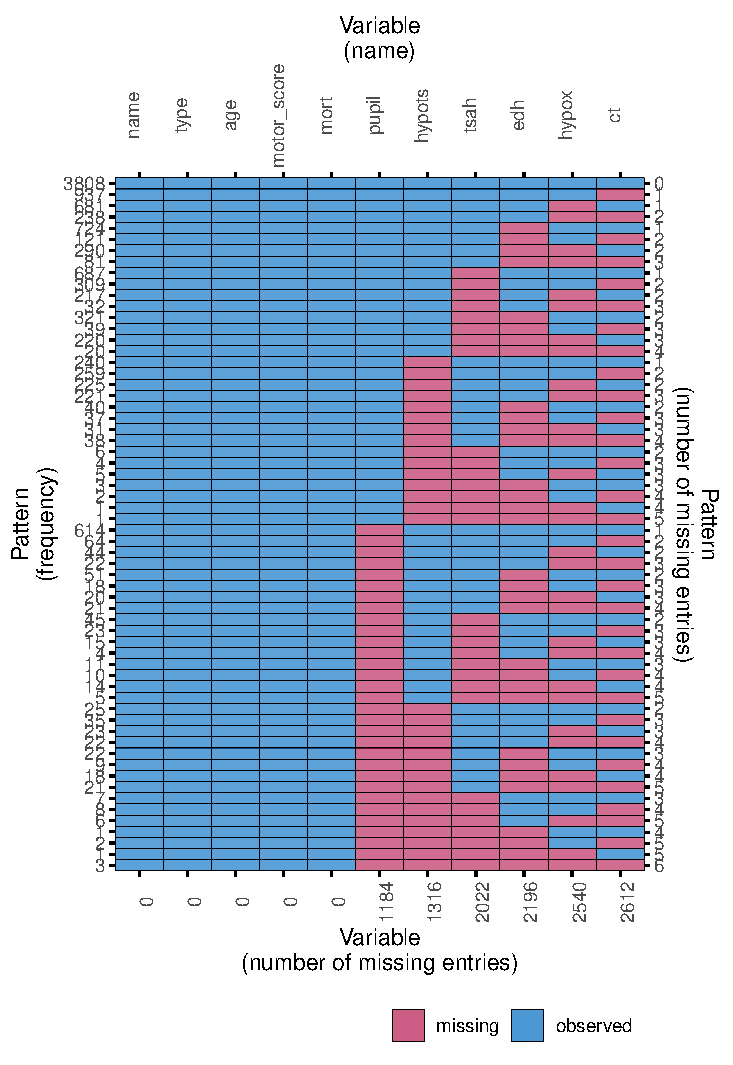
\includegraphics{Imputation_of_Incomplete_Multilevel_Data_files/figure-latex/pattern-1} \end{center}

\end{CodeChunk}

This shows that we need to impute \texttt{ct} and \texttt{pupil}.

To develop the best imputation model, we need to investigate the
relations between the observed values of the incomplete variables and
the observed values of other variables, and the relation between the
missingness indicators of the incomplete variables and the observed
values of the other variables. To see whether the missingness depends on
the observed values of other variables, we can test this statistically
or use visual inspection (e.g.~a histogram faceted by the missingness
indicator).

We should impute the variables \texttt{ct} and \texttt{pupil} and any
auxiliary variables we might want to use to impute these incomplete
analysis model variables. We can evaluate which variables may be useful
auxiliaries by plotting the pairwise complete correlations:

\begin{CodeChunk}
\begin{CodeInput}
R> plot_corr(dat, rotate = TRUE) # plot correlations 
\end{CodeInput}


\begin{center}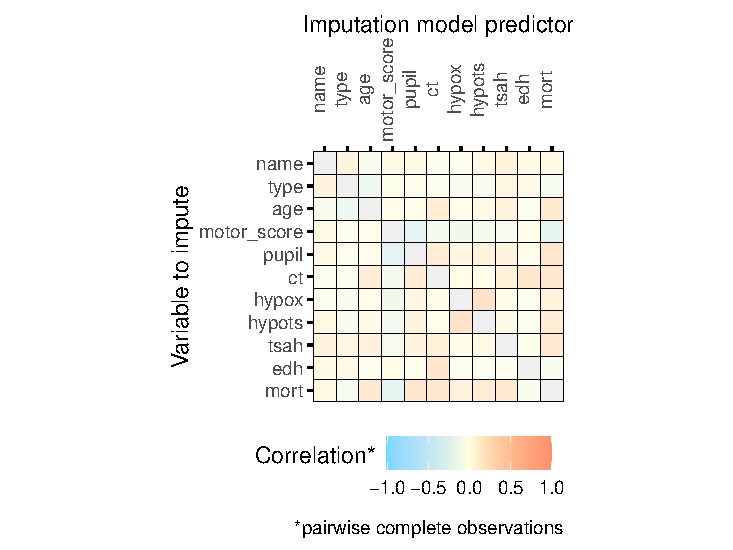
\includegraphics{Imputation_of_Incomplete_Multilevel_Data_files/figure-latex/impact_corr-1} \end{center}

\end{CodeChunk}

This shows us that \texttt{hypox} and \texttt{hypot} would not be useful
auxiliary variables for imputing \texttt{ct}. Depending on the minimum
required correlation, \texttt{tsah} could be useful, while \texttt{edh}
has the strongest correlation with \texttt{ct} out of all the variables
in the data and should definitely be included in the imputation model.
For the imputation of \texttt{pupil}, none of the potential auxiliary
variables has a very strong relation, but \texttt{hypots} could be used.
We conclude that we can exclude \texttt{hypox} from the data, since this
is neither an analysis model variable nor an auxiliary variable for
imputation:

\begin{CodeChunk}
\begin{CodeInput}
R> dat <- select(dat, !hypox)  # remove variable
R> dat <- mutate(dat, motor_score = as.factor(motor_score))
\end{CodeInput}
\end{CodeChunk}

\hypertarget{complete-case-analysis}{%
\subsection{Complete case analysis}\label{complete-case-analysis}}

As previously stated, complete case analysis lowers statistical power
and may bias results. The complete case analysis estimates are:

\begin{CodeChunk}
\begin{CodeInput}
R> fit <- glmer(mod, family = "binomial", data = na.omit(dat)) # fit the model
R> tidy(fit, conf.int = TRUE, exponentiate = TRUE)             # print estimates
\end{CodeInput}
\begin{CodeOutput}
# A tibble: 11 x 9
   effect  group term  estimate std.error statistic   p.value conf.low conf.high
   <chr>   <chr> <chr>    <dbl>     <dbl>     <dbl>     <dbl>    <dbl>     <dbl>
 1 fixed   <NA>  (Int~   0.0863   0.0182     -11.6   3.00e-31   0.0571     0.130
 2 fixed   <NA>  type~   0.757    0.137       -1.54  1.22e- 1   0.531      1.08 
 3 fixed   <NA>  age     1.03     0.00265     12.9   7.40e-38   1.03       1.04 
 4 fixed   <NA>  moto~   0.651    0.0732      -3.82  1.34e- 4   0.522      0.811
 5 fixed   <NA>  moto~   0.489    0.0555      -6.30  2.97e-10   0.391      0.611
 6 fixed   <NA>  moto~   0.274    0.0321     -11.0   2.28e-28   0.218      0.345
 7 fixed   <NA>  pupi~   3.20     0.317       11.7   8.18e-32   2.63       3.88 
 8 fixed   <NA>  pupi~   1.75     0.195        5.06  4.27e- 7   1.41       2.18 
 9 fixed   <NA>  ctIII   2.41     0.268        7.89  3.05e-15   1.94       2.99 
10 fixed   <NA>  ctIV~   2.30     0.214        8.95  3.56e-19   1.92       2.76 
11 ran_pa~ name  sd__~   0.230   NA           NA    NA         NA         NA    
\end{CodeOutput}
\end{CodeChunk}

As we can see, a higher \texttt{ct} (Marshall Computerized Tomography
classification) is associated with a lower odds of 6-month mortality,
given by the odds ratio exp(0.42), CI \ldots{} to \ldots, when
controlling for\ldots{}

\hypertarget{imputation-model}{%
\subsection{Imputation model}\label{imputation-model}}

Mutate data to get the right data types for imputation (e.g.~integer for
clustering variable).

\begin{CodeChunk}
\begin{CodeInput}
R> dat <- dat %>% mutate(across(everything(), as.integer))
\end{CodeInput}
\end{CodeChunk}

Create a methods vector and predictor matrix, and make sure
\texttt{name} is not included as predictor, but as clustering variable:

\begin{CodeChunk}
\begin{CodeInput}
R> meth <- make.method(dat) # methods vector
R> pred <- quickpred(dat)   # predictor matrix
R> plot_pred(pred, rotate = TRUE)
\end{CodeInput}


\begin{center}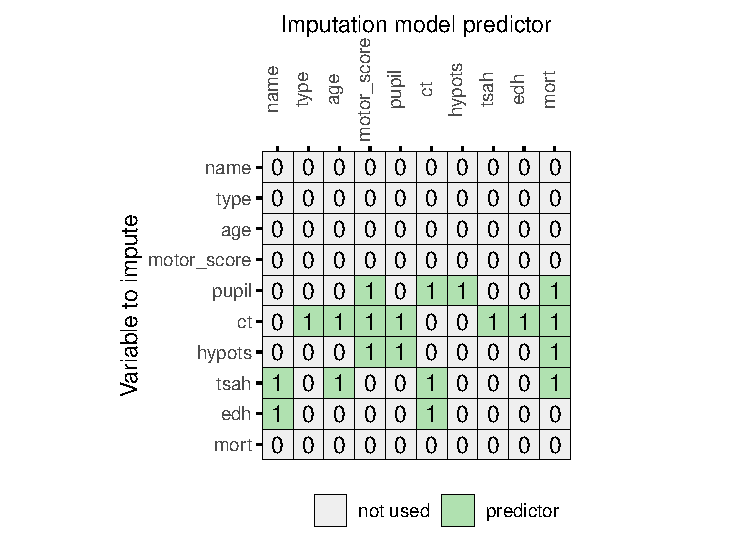
\includegraphics{Imputation_of_Incomplete_Multilevel_Data_files/figure-latex/impact-1} \end{center}

\begin{CodeInput}
R> pred[pred == 1] <- 2
R> pred["mort", ] <- 2
R> pred[, "mort"] <- 2
R> pred[c("name", "type", "age", "motor_score", "mort"), ] <- 0
R> pred[, "name"] <- -2
R> diag(pred) <- 0
R> plot_pred(pred, rotate = TRUE)
\end{CodeInput}


\begin{center}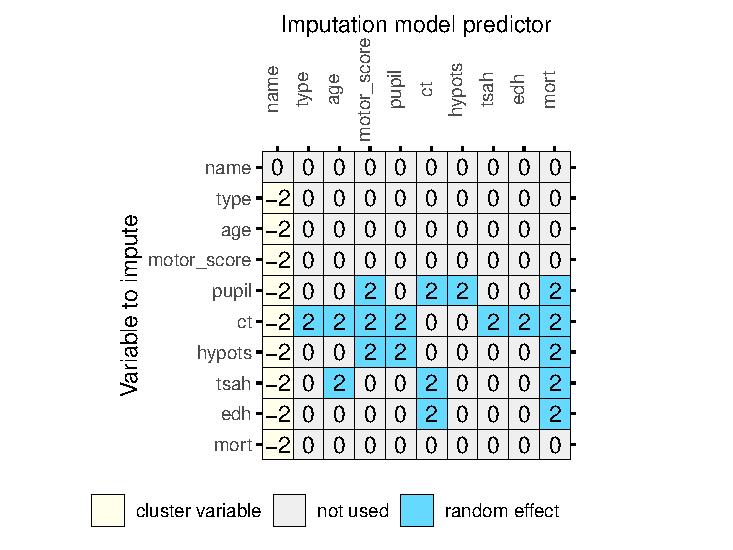
\includegraphics{Imputation_of_Incomplete_Multilevel_Data_files/figure-latex/impact-2} \end{center}

\begin{CodeInput}
R> meth <- make.method(dat)
R> meth
\end{CodeInput}
\begin{CodeOutput}
       name        type         age motor_score       pupil          ct 
         ""          ""          ""          ""       "pmm"       "pmm" 
     hypots        tsah         edh        mort 
      "pmm"       "pmm"       "pmm"          "" 
\end{CodeOutput}
\end{CodeChunk}

Impute the incomplete data

\begin{CodeChunk}
\begin{CodeInput}
R> imp <- mice(dat, method = meth, predictorMatrix = pred, printFlag = FALSE)
\end{CodeInput}
\end{CodeChunk}

Evaluate the convergence of the algorithm:

\begin{CodeChunk}
\begin{CodeInput}
R> plot_trace(imp)
\end{CodeInput}


\begin{center}\includegraphics{Imputation_of_Incomplete_Multilevel_Data_files/figure-latex/impact-conv-1} \end{center}

\end{CodeChunk}

Analyze the imputed data:

\begin{CodeChunk}
\begin{CodeInput}
R> fit <- imp %>% 
+   with(glmer(
+     mort ~ type + age + as.factor(motor_score) + pupil + ct + (1 | name),
+     family = "binomial"
+     )) 
R> # tidy(pool(fit))
R> # as.mitml.result(fit)
R> # testEstimates(as.mitml.result(fit))
\end{CodeInput}
\end{CodeChunk}

The estimated effects after imputation are presented in Table XYZ.

\hypertarget{case-study-iii-obesity-data}{%
\section{Case study III: obesity
data}\label{case-study-iii-obesity-data}}

In this example, we demonstrate a multilevel imputation of random
intercept and random slope model with a continuous response. We utilize
the obesity dataset included in the \texttt{micemd}@ package, a
simulated dataset that emulates an electronic survey in which
individuals are asked to provide information about their weight and
consumption habits in different countries. We simulate data for 5
clusters so that the true values are known. We use the following
variables from the dataset:

\begin{itemize}
\tightlist
\item
  \textbf{Cluster:} Region of the patients' healthcare provider (Cluster
  variable),
\item
  \textbf{Gender:} Subjects' Gender (0=male, 1=female),
\item
  \textbf{Age:} Subjects' age,
\item
  \textbf{Height:} Subjects' height in metres,
\item
  \textbf{Weight:} Subjects' weight in kilograms,
\item
  \textbf{BMI:} Subjects' body mass index,
\item
  \textbf{FamOb:} Family obesity history (yes or no),
\item
  \textbf{Time:} Response time in minutes (exclusion-restriction
  variable).
\end{itemize}

In this dataset, Age and FamOb are MAR, while the weight variable is
affected by selection bias, attributed to an indirect MNAR mechanism.
This MNAR mechanism typically arises when an unobserved or omitted
variable influences both the value of the incomplete variable (in this
case, Weight) and its likelihood of being missing (denoted as R).

In the primary analysis model, BMI serves as the dependent variable,
with Age, Gender, and FamOb as predictors. Because of the clustered
nature of the data, which is quantified with the Intraclass Correlation
Coefficient (ICC) below, we include random intercepts, as well as a
random slope for the Age variable. The model is represented as:
\begin{equation}
\label{eqn:main}
BMI_{ij}= (\beta_{o}+ b_{oj} ) + (\beta_{1}+ b_{oj})* Age_{ij} + \beta_{2}*FamOb_{ij}+ \beta_{3}Gender_{ij} + \epsilon_{ij}
\end{equation}

We start by loading the data:

\begin{CodeChunk}
\begin{CodeInput}
R> #data("data_heckman", package = "micemd")
R> #dat <- data_heckman
\end{CodeInput}
\end{CodeChunk}

Now, let's begin by examining the missing patterns in the data by
cluster:

\begin{CodeChunk}
\begin{CodeInput}
R> #ggmice::plot_pattern(data=Obesity,cluster="Cluster") does not work!! bug
R> #ggmice::plot_pattern(data=Obesity,cluster=Obesity$Cluster) does not work!! bug
R> library(ggpubr)
R> myplots <- lapply(1:5, function(i) {
+   ggmice::plot_pattern(setDT(Obesity)[Cluster==i])+
+   ggplot2::ggtitle(paste0("Cluster", i))
+  })
R> ggarrange(myplots[[1]], myplots[[3]], nrow=1,common.legend = TRUE, legend="bottom")
\end{CodeInput}
\begin{figure}

{\centering 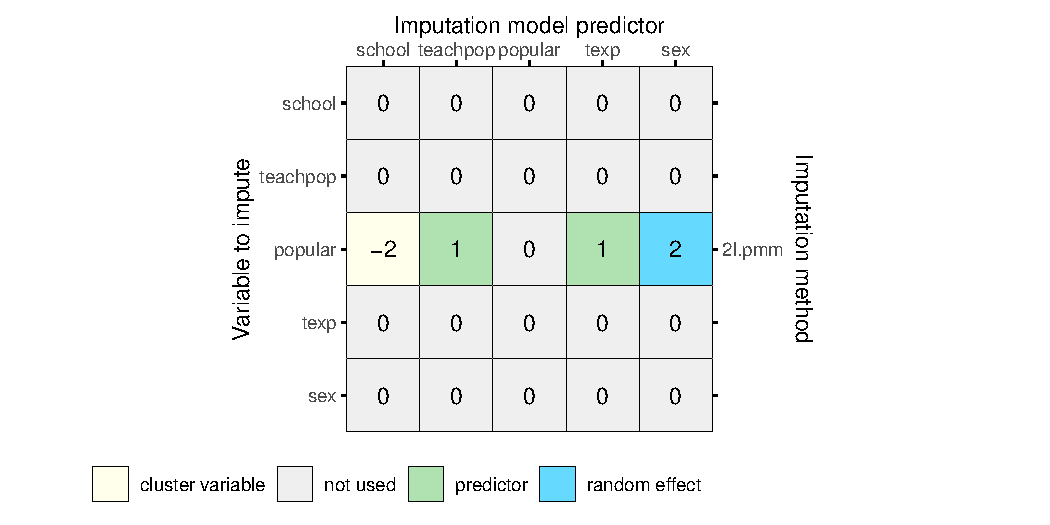
\includegraphics[width=0.7\linewidth]{Imputation_of_Incomplete_Multilevel_Data_files/figure-latex/unnamed-chunk-12-1} 

}

\caption[Missing pattern]{Missing pattern}\label{fig:unnamed-chunk-12}
\end{figure}
\end{CodeChunk}

We observe that the missing pattern is non-monotonic and quite similar
across the clusters. However, regarding the weight variable, we notice
that is systematically missing in cluster 3. In order to evaluate if we
require a imputation method that accounts for clustering we assess the
Intraclass Correlation

\begin{CodeChunk}
\begin{CodeInput}
R> Nulmodel <- lme4::lmer(BMI ~ 1 + (1|Cluster), data = Obesity)
R> performance::icc(Nulmodel)
\end{CodeInput}
\begin{CodeOutput}
# Intraclass Correlation Coefficient

    Adjusted ICC: 0.362
  Unadjusted ICC: 0.362
\end{CodeOutput}
\end{CodeChunk}

Since the ICC is above 0.1 and as the main analysis will be use a mixed
model, we decide to use two-level (2l) imputation methods. In this
imputation process, we include all predictor variables from equation
\ref{eqn:main} in the main model. However, since BMI is a composite of
weight and height, we use deterministic imputation for these, which is
described below.

We use the \textbf{find.defaultMethodfunction} provided in the
\textbf{micemd} package, which suggests an appropriate method for MAR
variables based on the type of variable, number of observations in the
cluster, and number of clusters.

It suggests using `2l.2stage.bin' for the FAV variable and
`2l.2stage.norm' for the age variable. However, after inspecting the age
density plot, we consider modifying its method to `2l.2stage.pmm'. For
the BMI variable, we employ deterministic imputation.

\begin{CodeChunk}
\begin{CodeInput}
R> library(micemd)
R> meth_mar <- micemd::find.defaultMethod(Obesity, ind.clust=1, I.small = 7,
+                                ni.small = 100, prop.small = 0.4)
R> meth_mar["BMI"]<- "~ I(Weight / (Height)^2)"
R> meth_mar["Age"]<-"2l.2stage.pmm" 
\end{CodeInput}
\end{CodeChunk}

For these imputation models, it is necessary to specify the prediction
matrix, with the cluster variable labelled as -2 and the predictor
variable measured within clusters labelled as 2, encompassing all
variables. We need to suprime the variable Time as this variable is not
specified in the main model. We also modify the relationship between
BMI, weight and height in the prediction matrix to avoid circular
predictions. Then we proceed to run the imputation model.

\begin{CodeChunk}
\begin{CodeInput}
R> pred_mar <- mice(Obesity, maxit = 0)$pred 
R> pred_mar[,"Cluster"] <- -2 # clustering variable
R> pred_mar[,"Time"] <- 0
R> pred_mar[pred_mar==1] <- 2
R> pred_mar[c("Height", "Weight"), "BMI"] <- 0
R> ggmice::plot_pred(pred_mar)
\end{CodeInput}


\begin{center}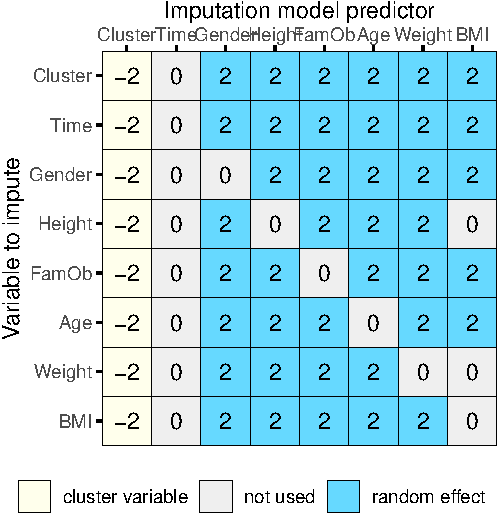
\includegraphics[width=0.7\linewidth]{Imputation_of_Incomplete_Multilevel_Data_files/figure-latex/obesity-predmar-1} \end{center}

\begin{CodeInput}
R> imp_mar <- mice::mice(data = Obesity, meth = meth_mar, pred = pred_mar,
+                 m=10, seed = 123, printFlag = FALSE)
\end{CodeInput}
\end{CodeChunk}

\begin{CodeChunk}
\begin{CodeInput}
R> summary(complete(imp_mar,"long")$Weight)
\end{CodeInput}
\begin{CodeOutput}
   Min. 1st Qu.  Median    Mean 3rd Qu.    Max. 
 -19.48   68.45   81.65   81.28   94.12  160.76 
\end{CodeOutput}
\end{CodeChunk}

We are also contemplating the utilisation of the ???pmm??? option, as
the values imputed using a fully parametric method may be implausibly
low for some patients.

\begin{CodeChunk}
\begin{CodeInput}
R> meth_mar["Weight"]<-"2l.2stage.pmm" 
R> imp_mar_pmm <- mice(data = Obesity, meth = meth_mar, pred = pred_mar,
+                     m=10, seed = 123, printFlag = FALSE)
\end{CodeInput}
\end{CodeChunk}

\begin{CodeChunk}
\begin{CodeInput}
R> summary(complete(imp_mar_pmm,"long")$Weight)
\end{CodeInput}
\begin{CodeOutput}
   Min. 1st Qu.  Median    Mean 3rd Qu.    Max. 
  28.35   69.25   82.43   82.41   94.76  134.61 
\end{CodeOutput}
\begin{CodeInput}
R> ggmice::plot_trace(imp_mar_pmm, "Weight")
\end{CodeInput}


\begin{center}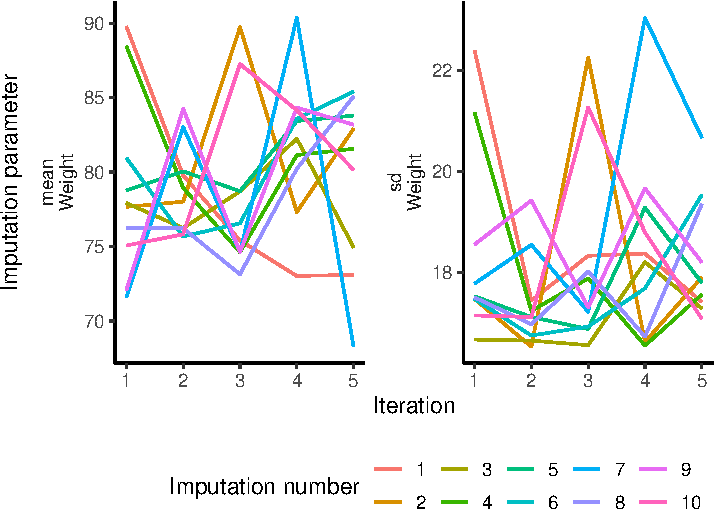
\includegraphics{Imputation_of_Incomplete_Multilevel_Data_files/figure-latex/obesity-predmar_pmm1-1} \end{center}

\end{CodeChunk}

After confirming convergence, we proceed to save the results for future
use. We consider the possibility that patients may not have been
selected randomly, which would then have led to a distribution for
weight that does not reflect the weight in the population. It???s likely
that an omitted variable, like self-esteem, could influence this
selection. For instance, individuals with lower self-esteem might have
higher weight values, impacting their willingness to provide honest
information due to embarrassment.

To address this situation, two approaches have been proposed for dealing
with Missing Not at Random (MNAR) data: pattern-mixed models and
selection models. Within pattern-mixed models, methods like the delta
method and more advanced ones like NARFS have been suggested. The
selection model approach includes methods such as the Heckman model,
which can be particularly useful in this case. Several methods,
including those by \cite{Galimar_2017,Hammon_2021}, and the recently a
Heckman method designed for two-level data, allow for variations in
intercepts and exposure effects (random intercept and slope).

To apply the \textbf{2l.2stage.heckman} method, the weight variable
should be specified as `2l.2stage.heckman' found in the micemd package.
Additionally, the prediction matrix needs modification because this
method involves specifying two equations: one for the outcome,
describing the incomplete variable in terms of partially observed
predictors (in this case, all variables from the main model), and the
other for the selection model, explaining the probability of being
observed based (R) on certain variables. For the outcome equation we
consider the same imputation model that we used for the MAR case (main
model).
\[Weight_{ij}= \beta^O_{o} + \beta^O_{1}Age_{ij} + \beta^O_{2}FamOb_{ij}+ \beta^O_{3}Gender_{ij} + \epsilon^O_{ij}\]
Regarding the selection equation, we include the same predictors as
those in the main model, as well as a time variable. Here the time
variable serves as a restriction exclusion variable specifically
explaining the probability of being observed but not affecting the
incomplete value (Weight). In this context, we assume that the time a
user spends completing the survey serves as a proxy for the barriers
they may encounter in survey completion, such as familiarity with the
survey content or internet speed. These factors may lead the user to
skip specific questions or even the entire survey. Also, we assume the
time does not have any influence on the subject???s weight.
\[R_{ij}= \beta^S_{o} + \beta^S_{1}Age_{ij} + \beta^S_{2}FamOb_{ij}+ \beta^S_{3}Gender_{ij} +\beta^S_{4}Time_{ij}+ \epsilon^S_{ij}\]

These two equations are jointly estimated under the assumption that the
error terms are interconnected with a bivariate normal distribution. For
a more comprehensive understanding of the model and the exclusion
restriction, see \cite{Munoz_2022}.

To use information from both equations, we must adjust the prediction
matrix. The cluster variable remains specified as before (-2). In this
imputation method, all the variables present in both the selection and
outcome equations are included with a random effect.

However, it is essential to distinguish which of these variables appear
in each equation. In this framework, when a variable is shared between
both equations, it is denoted as (2). Predictors exclusive to the
outcome equation are indicated as (-4), while those exclusive to the
selection equation are labelled as (-3). Consequently, the only
alteration needed in the predictor matrix pertains to the variable
`Time'.

\begin{CodeChunk}
\begin{CodeInput}
R> pred_mnar <- pred_mar
R> pred_mnar["Weight","Time"]<- -3
R> ggmice::plot_pred(pred_mnar)
\end{CodeInput}


\begin{center}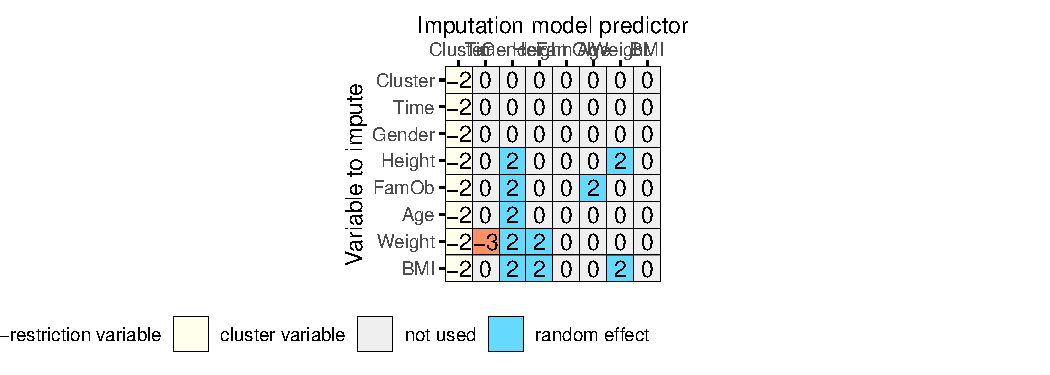
\includegraphics{Imputation_of_Incomplete_Multilevel_Data_files/figure-latex/obesity-predmnar-1} \end{center}

\end{CodeChunk}

We also need to modify the method of the weight variable.

\begin{CodeChunk}
\begin{CodeInput}
R> meth_mnar <- meth_mar
R> meth_mnar["Weight"]<- "3l.2stage.heckman"
\end{CodeInput}
\end{CodeChunk}

Then we proceed to run the imputation model as before, after executing
these imputation procedures, it is essential to assess convergence and
the coherence of the imputed values.

\begin{CodeChunk}
\begin{CodeInput}
R> imp_mnar<- mice(data = Obesity, meth = meth_mnar, pred = pred_mnar,
+                 m=10, seed = 123, printFlag = FALSE)
R> summary(complete(imp_mnar,"long")$Weight)
\end{CodeInput}
\begin{CodeOutput}
   Min. 1st Qu.  Median    Mean 3rd Qu.    Max. 
  14.09   71.68   85.33   85.79   99.31  186.67 
\end{CodeOutput}
\end{CodeChunk}

Upon examining the weight variable, we noticed that the imputed range
falls outside the realm of plausible values (as weight should be
positive).

\begin{CodeChunk}
\begin{CodeInput}
R> summary(complete(imp_mnar,"long")$Weight)
\end{CodeInput}
\begin{CodeOutput}
   Min. 1st Qu.  Median    Mean 3rd Qu.    Max. 
  14.09   71.68   85.33   85.79   99.31  186.67 
\end{CodeOutput}
\end{CodeChunk}

Consequently, as before we use the `pmm', option but this time for the
Heckman imputation, this approach ensures that the imputed values remain
within the range of observable values. We then run the imputation model
but this time using the option of pmm, to assure that weight values are
in the range of the observable data, this can be implemented by setting
the pmm parameter to true.

\begin{CodeChunk}
\begin{CodeInput}
R> imp_mnar_pmm <- mice(data = Obesity, meth = meth_mnar, pred = pred_mnar,
+                      m=10, seed = 123, pmm = T,  printFlag = FALSE)
\end{CodeInput}
\end{CodeChunk}

We check the convergency of the results

\begin{CodeChunk}
\begin{CodeInput}
R> summary(complete(imp_mnar_pmm,"long")$Weight)
\end{CodeInput}
\begin{CodeOutput}
   Min. 1st Qu.  Median    Mean 3rd Qu.    Max. 
  28.35   71.51   85.09   85.64   99.00  134.61 
\end{CodeOutput}
\begin{CodeInput}
R> ggmice::plot_trace(imp_mar_pmm, "Weight")
\end{CodeInput}


\begin{center}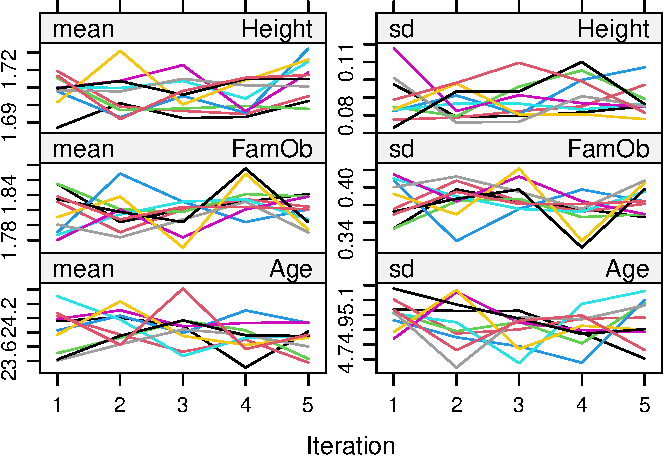
\includegraphics{Imputation_of_Incomplete_Multilevel_Data_files/figure-latex/obesity-predmnarp1-1} \end{center}

\end{CodeChunk}

After this modification we proceed to compare the effects on the model.
We run the analysis model on each of the completed datasets as well
asthe dataset where the incomplete values are removed (Complete Case
analysis, CC).

\begin{CodeChunk}
\begin{CodeInput}
R> library(ggplot2)
R> cc_rs<- with(setDT(Obesity)[complete.cases(Obesity),],
+              lme( BMI ~ Age + FamOb + Gender, random=~1+Age|Cluster))
R> mar_rs <- with(imp_mar,lme( BMI ~ Age + FamOb + Gender,random=~1+Age|Cluster))
R> mar_pmm_rs <- with(imp_mar_pmm,lme( BMI ~ Age + FamOb + Gender,random=~1+Age|Cluster))
R> mnar_rs<- with(imp_mnar,lme(BMI ~ Age + FamOb + Gender,random=~1+Age|Cluster))
R> mnar_pmm_rs<- with(imp_mnar_pmm, lme(BMI ~ Age + FamOb + Gender,random=~1+Age|Cluster))
R> list_models<-list(cc_rs,mar_rs,mar_pmm_rs,mnar_rs,mnar_pmm_rs)
R> plot_models(list_models,
+             mod_name = c("Complete case", "MAR","MAR_pmm", "MNAR", "MNAR_pmm"))
\end{CodeInput}


\begin{center}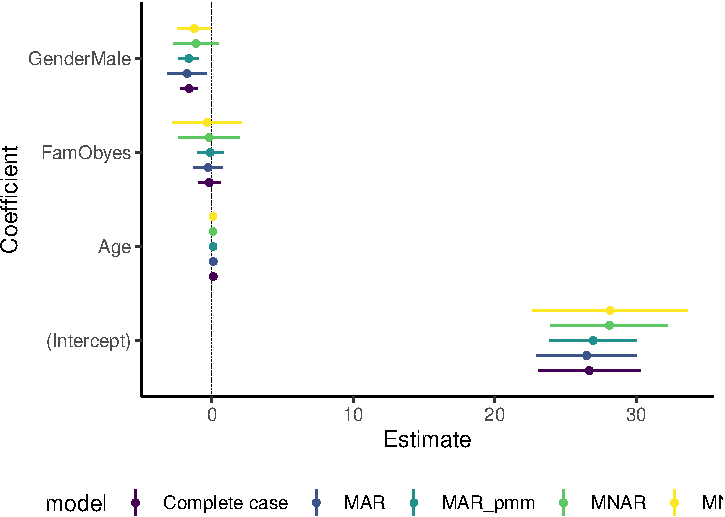
\includegraphics{Imputation_of_Incomplete_Multilevel_Data_files/figure-latex/models-1} \end{center}

\end{CodeChunk}

We note that there is minimal disparity in the age effect, FamObs, or
Gender across the various imputation models under consideration. An
analysis of the intercept reveals that, under the MNAR assumption, a
higher average BMI is anticipated compared to the MAR assumption.
Nonetheless, with respect to precision of estimates, we notice that in
general MNAR imputation leads to wider confidence intervals, in this
case it does not have any influence on the final result but there could
be cases where variation in the assumed missing mechanism could lead
also to differences on significant test and therefore lead to
contradictory conclusions.

\hypertarget{additional}{%
\section{Additional}\label{additional}}

The imputation of these data is based on the
\href{https://github.com/johamunoz/Heckman-IPDMA/blob/main/Toy_example.R}{IPDMA
Heckman Github repo}

Visualize missing data pattern:

The matrix only shows the predictors for the main model, not the
selection model.

TODO: explain exclusion restriction.

ORDER:

\begin{itemize}
\item
  summary
\item
  congeniality, then in hierarchical models
\item
  look whether we can fit cong. back in the main body
\item
  alt. methods
\item
  conclusion: mice is really easy!
\item
  Additional levels of clustering
\item
  More complex data types: timeseries and polynomial relationship in the
  clustering.
\item
  FIML vs MI
\end{itemize}

An alternative approach to missing data is to use Full Information
Maximum Likelihood (FIML). This method does not require the imputation
of any missing values. Whereas MI consists of imputation, analyses and
pooling steps, FIML analyses the data in a single step. When the
assumptions are met the two approaches should produce equivalent
results. {[}REF{]} As FIML requires specialised software, not all
analyses can be performed with standard software. {[}REF{]}

\begin{itemize}
\tightlist
\item
  Survival / TTE, this could be put in the paragraph on congeniality
\end{itemize}

When the outcome is time-to-event, the Nelson-Aalen estimate of the time
to event should be included as a covariate in the imputation model
{[}REF{]}

ORDER:

\begin{itemize}
\item
  summary
\item
  congeniality, then in hierarchical models
\item
  look whether we can fit cong. back in the main body
\item
  alt. methods
\item
  conclusion: mice is really easy!
\item
  Additional levels of clustering
\item
  More complex data types: timeseries and polynomial relationship in the
  clustering.
\item
  FIML vs MI
\end{itemize}

An alternative approach to missing data is to use Full Information
Maximum Likelihood (FIML). This method does not require the imputation
of any missing values. Whereas MI consists of imputation, analyses and
pooling steps, FIML analyses the data in a single step. When the
assumptions are met the two approaches should produce equivalent
results. {[}REF{]} As FIML requires specialised software, not all
analyses can be performed with standard software. {[}REF{]}

\begin{itemize}
\tightlist
\item
  Survival / TTE, this could be put in the paragraph on congeniality
\end{itemize}

When the outcome is time-to-event, the Nelson-Aalen estimate of the time
to event should be included as a covariate in the imputation model
{[}REF{]}

In hierarchical datasets, clustering is a concern because the
homoscedasticity in the error terms cannot be assumed across clusters
and the relationship among variables may vary at different hierarchical
levels. When multiple imputation is used to deal with missing data, as
the imputation and analysis process is performed separately, it is
necessary that imputation model being congenial with the main analysis
model (Meng, 1994), e.g.~if the main model accounts for the hierarchical
structure also imputation model should do it (Audigier, 2021). Not
including clustering into the imputation process may lead to effect
estimates with smaller standard errors and inflated type I error.

There are different strategies that can be adopted in the imputation
process that account for clustering: inclusion of cluster indicator
variable, performing a separate imputation process for each cluster, or
performing a simultaneous imputation process by using an imputation
method that accounts for clustering.(Stata:
\url{https://www.stata.com/support/faqs/statistics/clustering-and-mi-impute/})
TODO: replace ref.

The selection of each strategy depends mainly on the assumptions in the
main analysis and also on the restriction of the analyzed data.

Regarding the restrictions imposed by the data, for instance, the use of
cluster indicator variables is restricted in datasets where there are
not many clusters and many observations per cluster (Graham, 2009). The
last restriction is also required when imputations are performed on each
cluster separately. When this restriction cannot be achieved, one can
use an imputation model that simultaneously imputes all clusters using a
hierarchical model (Allison 2002).

Under this hierarchical imputation model, observations within clusters
are correlated and this correlation is modeled by a random effect so the
hierarchical model can be estimated even when there are few observations
per cluster. However, this strategy is best suited for balanced data
(Grund, 2017) and when random effects model is appropriated, i.e.~the
number of clusters is adequate. (Austin,2018).

Here it is important to evaluate the assumptions imposed by the main
model, for instance by using the cluster indicator strategy may lead to
bias estimates when the model is based on a hierarchical model
(Taaljard,2008). Even when an imputation strategy congenial with the
main model is preferred, it is important to consider whether it is
appropriate for the data as a less complex imputation strategies may
also lead to unbiased estimates in certain scenarios(Bailey 2020). For
instance, in causal effect analysis, separately imputation may lead to
smaller bias when the size of the smaller exposure cluster is large,
compared with an imputation model that includes exposure-confounder
interactions. (Zhang,2023).

\hypertarget{conclusion}{%
\section{Conclusion}\label{conclusion}}

\hypertarget{funding}{%
\section{Funding}\label{funding}}

This project has received funding from the European Union's Horizon 2020
research and innovation programme under ReCoDID grant agreement No
825746.

The views expressed in this paper are the personal views of the authors
and may not be understood or quoted as being made on behalf of or
reflecting the position of the regulatory agency/agencies or
organizations with which the authors are employed/affiliated.

\hypertarget{references}{%
\section{References}\label{references}}

\hypertarget{appendix}{%
\section{Appendix}\label{appendix}}

Table 3: Notation

\begin{longtable}[]{@{}
  >{\raggedright\arraybackslash}p{(\columnwidth - 2\tabcolsep) * \real{0.5495}}
  >{\raggedright\arraybackslash}p{(\columnwidth - 2\tabcolsep) * \real{0.4505}}@{}}
\toprule\noalign{}
\begin{minipage}[b]{\linewidth}\raggedright
\textbf{Formula \pkg{lme4}}
\end{minipage} & \begin{minipage}[b]{\linewidth}\raggedright
\textbf{Details}
\end{minipage} \\
\midrule\noalign{}
\endhead
\bottomrule\noalign{}
\endlastfoot
\texttt{y\ \textasciitilde{}\ x1\ +\ (1\ \textbar{}\ g1)} & Fixed
\texttt{x1} predictor with random intercept \\
& varying among \texttt{g1} \\
\texttt{y\textasciitilde{}x1*x2+\ (1\textbar{}\ g1)} & Interactions of
\texttt{x1} and \texttt{x2} only in fixed effect \\
\texttt{y\ \textasciitilde{}\ x1*x2+\ (x2\textbar{}\ g1)} & Interactions
of \texttt{x1} and \texttt{x2} only in fixed effect \\
& with slope of \texttt{x2} randomly varying among \texttt{g1} \\
\texttt{y\ \textasciitilde{}\ x1*x2+\ (x1*x2\textbar{}\ g1)} &
variance-covariance matrix estimated only with \\
& the variance terms of intercept, slope of \texttt{x1}, \\
& slope of \texttt{x2} and interaction \texttt{x1*x2} \\
\texttt{y\ \textasciitilde{}\ x1*x2+\ (x1\ \textbar{}\ g1)+\ (x2\textbar{}\ g1)}
& variance-covariance matrix estimated separately, \\
& i.e, one for intercept and \texttt{x1} and another for \\
& intercept and \texttt{x2} \\
\texttt{y\ \textasciitilde{}\ x1\ +\ (x1\ \textbar{}\ g1)\ or\ 1\ +\ x1\ +\ (1\ +\ x1\ \textbar{}\ g1)}
& Fixed \texttt{x1} with correlated random intercept and \\
& random slope of \texttt{x} \\
\texttt{y\ \textasciitilde{}\ x1\ +\ (x1\ \textbar{}\textbar{}\ g1)\ or\ 1\ +\ x1\ +\ (1\ \textbar{}\ g1)\ +\ (0\ +\ x1\ \textbar{}\ g1)}
& Fixed \texttt{x1} with uncorrelated random intercept \\
& and random slope of \texttt{x1} \\
\texttt{y\ \textasciitilde{}\ (1\ \textbar{}\ g1)\ +\ (1\ \textbar{}\ g2)}
& Random intercept varying among \texttt{g1} and among
\texttt{g2\ \ \ \textbar{}\ \textbar{}}y \textasciitilde{} (1 \\
& \\
\end{longtable}

\bibliography{../References/multilevelmice.bib}



\end{document}
